\section{Calculating potentials of mean force: the pull code}
\label{sec:pull}
There are a number of options to calculate \swapindex{potentials
of}{mean force}\index{force, potential of mean|see{potentials of mean force}}
\index{free energy calculations}
and related topics. In the current version of {\gromacs} this is
implemented through some extra files for {\tt mdrun}. 

\subsection{Overview}
Four different types of calculation are supported:

\begin{enumerate}
\item{\textbf{Constraint forces}} The distance between the centers of
mass of two groups of atoms can be constrained and the 
\swapindex{constraint}{force} monitored.
The distance can be in 1, 2, or 3 dimensions. This method
uses the SHAKE algorithm but only needs 1 iteration to be
exact if only two groups are constrained. 
\item{\textbf{Umbrella sampling}} A simple
\swapindex{umbrella}{sampling} with an
harmonic umbrella potential that acts on the center of mass of a group
of atoms.
\item{\textbf{\swapindex{AFM}{pulling}}} A spring is connected to an atom and
slowly retracted. This has the effect of pulling an atom or group of
atoms away from its initial location. The rate constant and spring
constant for the spring can be varied to study e.g. the unbinding of a
protein and a ligand (see figure~\ref{fi:pull}). 
\begin{figure}
\centerline{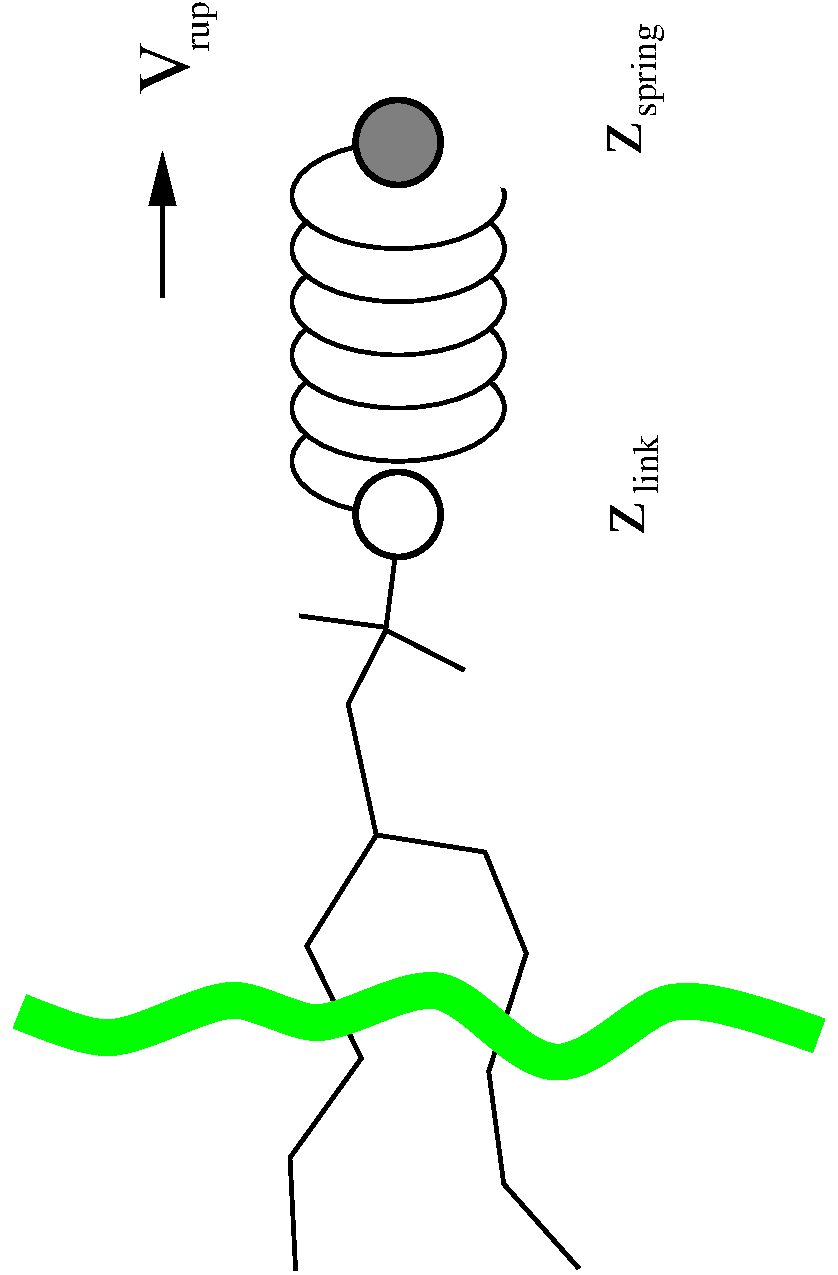
\includegraphics[width=6cm,angle=270]{plots/pull}}
\caption{Schematic picture of pulling a lipid out of a lipid bilayer
with AFM pulling. $V_{rup}$ is the velocity at which the spring is
retracted, $Z_{link}$ is the atom to which the spring is attached and
$Z_{spring}$ is the location of the spring.}
\label{fi:pull} 
\end{figure}   
\item{\textbf{Starting structures}} This option creates a number of
starting structures for potential of mean force calculations, moving 1
or 2 groups of atoms at a specified rate towards or away from a
reference group, writing out a coordinate file at specified intervals.
Note that the groups given in the index file are translated a
specified distance each step, but in addition also undergo the normal
MD, subject to definitions of \emph{e.g.} temperature coupling groups, freeze
groups and the like.
\end{enumerate}

In the calculations, there has to be 1 reference group and 1 or 2
other groups of atoms. For constrained runs, the distance between the
reference group and the other groups is kept constant at the distance
they have in the input coordinate file ({\tt .tpr}) file.

\subsection{Usage}

\subsubsection{Input files}

The {\tt mdrun} programs needs 4 additional files: 2 input files and 2
output files. 
\begin{description}
\item[\tt -pi pull.ppa]\mbox{}\\ If this file is specified the pull code will
be used. It contains the parameters that control what type of
calculation is done. A full explanation of all the options is given below.
\item[\tt -pn index.ndx]\mbox{}\\ This file defines the different groups for
use in all pull calculations. The groups are referred to by name, so
the index file can contain other groups that are not used as well. 
\item[\tt -po pullout.ppa]\mbox{}\\ A formatted copy of the input parameter
file with the parameters that were actually used in the run.
\item[\tt -pdo pull.pdo]\mbox{}\\ The data file with the calculated forces
(AFM pulling, constraint force) or positions (umbrella sampling).
\end{description}

\subsubsection{Definition of groups}

The way the reference groups and different reference types work is
summarized in figure~\ref{fi:pullref}. There are four different
possibilities for the reference group. 

\begin{figure}
\centerline{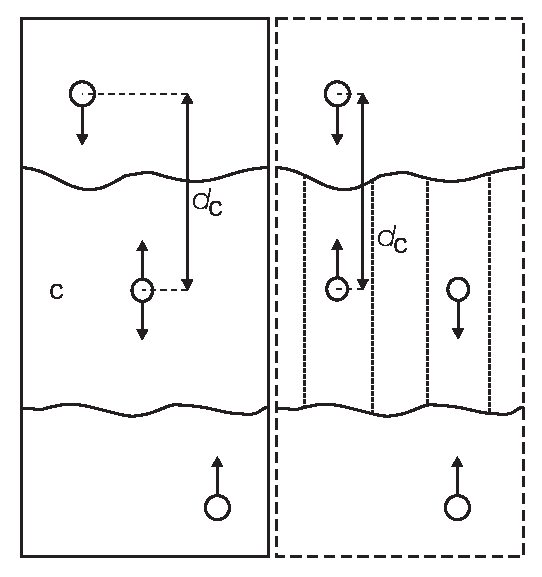
\includegraphics[width=6cm]{plots/pullref}}
\caption{Overview of the different reference group possibilities,
applied to interface systems. C is the reference group. The circles
represent the center of mass of 2 groups plus the reference group, and
$d_c$ is the reference distance.}
\label{fi:pullref} 
\end{figure}   

\begin{description}
\item[\tt com]\mbox{}\\ The center of mass of the group given under {\tt
reference\_group}, calculated each step from the current coordinates. 
\item[\tt com\_t0]\mbox{}\\ The center of mass of the group given under {\tt
reference\_group}, calculated each step from the current coordinates,
but corrected for atoms that have crossed the box. If the reference
group consists of all the water molecules in the system, and a single
water molecule moves across the box and enters from the other side,
the c.o.m. will show a slight jump. This is simply due to the periodic
boundary conditions, and shows that the center of mass in a simulation
in periodic boundary conditions is ill defined if the group
used to calculate it is \emph{e.g.} a slab of liquid. If the 'real'
positions are used instead of the coordinates that have been reset to
be inside the box, the center of mass of the \textbf{whole} system is 
conserved. 
\item[\tt dynamic]\mbox{}\\ In a phospholipid bilayer system it may be of
interest to calculate the pmf of a lipid as function of its distance
from the whole bilayer. The whole bilayer can be taken as reference
group in that case, but it might also be of interest to define the
reaction coordinate for the pmf more locally. {\tt dynamic} does not
use all the atoms of the {\tt reference\_group}, but instead only those
within a cylinder with radius {\tt r} below the main group. This only
works for distances defined in 1 dimension, and the cylinder is
oriented with its long axis along this 1 dimension. A second cylinder
can be defined with {\tt rc}, with a linear switch function that weighs
the contribution of atoms between {\tt r} and {\tt rc} with
distance. This smoothes the effects of atoms moving in and out of the
cylinder (which causes jumps in the constraint forces). 
\item[\tt dynamic\_t0]\mbox{}\\
The same as {\tt dynamic}, but using the coordinates corrected for
boxcrossings like in {\tt com\_t0}. Note that strictly speaking this is
not correct if the reference group is not the whole system, including
the groups defined with {\tt group\_1} and {\tt group\_2}.
\end{description}

To further smooth rapidly fluctuating distances between the reference
group and the other groups, the average distance can be constrained
instead of the instanteneous distance. This is defined by setting {\tt
reflag} to the number of steps to average over. However, using this
option is not strictly correct for calculating potentials of mean
force from the average constraint force. 

\subsubsection{The parameter file}

\begin{description}
\item[\tt verbose                  = no]\mbox{}\\
If this is set to {\tt yes}, a large amount of detailed information
is sent to {\tt stderr}, which is only useful for diagnostic
purposes. The {\tt .pdo} file also becomes more detailed, which is not
necessary for normal use.

\item[\tt runtype                  = constraint]\mbox{}\\
Options are {\tt start, afm, constraint, umbrella}. This selects the
type of calculation: making starting structures, AFM pulling,
constraint force calculation or umbrella sampling.

\item[\tt group\_1                  = MB21\_1]
\item[\tt group\_2                  = MB21\_2]\mbox{}\\                 
The groups with the atoms to act on. The first group is mandatory, the
second optional.

\item[\tt reference\_group          = OCTA]\mbox{}\\
The reference group. Distances are calculated betweeen {\tt group\_1}
(and {\tt group\_2} if specified) and this group. If \emph{e.g.} the
constraint force between two ions is needed, you would specifiy {\tt
group\_1} as a group with 1 ion, and {\tt reference\_group} as the other
ion.

\item[\tt reftype                  = com]\mbox{}\\
The type of reference group. Options are {\tt com, com\_t0, dynamic,
dynamic\_t0} as explained above. 

\item[\tt reflag                   = 1]\mbox{}\\
The position of the reference group can be taken as average over a
number of steps, specified by {\tt reflag} (see above).

\item[\tt direction                = 0.0 0.0 1.0]\mbox{}\\
Distances are calculated weighted by x, y, z as specified in {\tt
direction}. Setting them all to 1.0 calculates the distance between
two groups, setting the first two to 0.0 and the third to 1.0
calculates the distance in the z direction only.

\item[\tt reverse                  = to\_reference]\mbox{}\\
This option selects the direction in which the groups are moved with
respect to the reference group for AFM pulling and starting structure
calculations. The options are {\tt to\_reference, from\_reference}.

\item[\tt r                        = 0]\mbox{}\\
If dynamic reference groups are selected ({\tt dynamic, dynamic\_t0}),
{\tt r} is the radius of the cylinder used to define which atoms are
part of the reference group (see above).

\item[\tt rc                       = 0]\mbox{}\\
With dynamic reference groups, the cylinder can be smoothly switched
so that atoms that fall between {\tt r} and {\tt rc} are weighted
linearly from 1 to 0 going from {\tt r} to {\tt rc}. As reasonable
initial values we suggest {\tt r = 1.0} and {\tt rc = 1.5} but this
will depend strongly on the exact system of interest.

\item[\tt update                   = 1]\mbox{}\\
The frequency with which the dynamic reference groups are
recalculated. Usually there is no reason to use anything other than 1.

\item[\tt pullrate                 = 0.00005]\mbox{}\\
The pull rate in nm/timestep for AFM pulling.

\item[\tt forceconstant            = 100]\mbox{}\\
The force constant for the spring in AFM pulling, in kJ mol$^{-1}$
nm$^{-2}$.

\item[\tt width                    = 0]\mbox{}\\
Width of the umbrella sampling potential in kJ mol$^{-1}$ nm$^{-2}$. 

\item[\tt r0\_group2                = 0.0  0.0   3.300]\mbox{}\\
The initial location of the groups with respect to the reference
group. Only coordinates selected with {\tt direction} are taken into account.
The groups are moved to these initial positions before the
actual creation of a series of starting structures commences.

\item[\tt tolerance                = 0.001]\mbox{}\\
The accuracy with which the actual position of the groups must match
the calculated ideal positions for a starting structure (in nm).
 
\item[\tt translation\_rate         = 0.00001]\mbox{}\\
The rate of translation in all directions (nm/step). As mentioned
above, normal MD force calculations and position updates also act on
the groups.

\item[\tt transstep                = 0.2]\mbox{}\\
The interval in nm at which structures are written out. 

\end{description}

\subsection{Output}
The output file is a text file with forces or positions, one per
line. If there are two groups they alternate in the output
file. Currently there is no supported analysis program to read this
file, but it is simple to parse.

\subsection{Limitations}
Apart from obvious limitations that are simply not implemented (\emph{e.g.} a
better umbrella sampling and analysis scheme), there is one important
limitation: constraint forces can \textbf{only} be calculated between
molecules or groups of molecules. If a group contains part of a
molecule of which the bondlengths are constrained, SHAKE or LINCS and
the constraint force calculation here will interfere with each other,
making the results unreliable. If a constraint force is wanted between
two atoms, this can be done through the free energy perturbation
code. In summary: 

\begin{itemize}
\item{\bf pull code:} between molecules or groups of molecules.
\item{\bf free energy perturbation code:} between single atoms. 
\item{\bf not possible currently:} between groups of atoms that are
part of a larger molecule for which the bonds are constrained with
SHAKE or LINCS.
\end{itemize}

\subsection{Implementation}

The code for the options described above can be found in the files
{\tt pull.c, pullinit.c, pullio.c, pullutil.c} and the headerfiles
{\tt pull.h} and {\tt pulls.h}. This last file defines a few
datatypes, {\tt pull.h} explains the main functions. 

\subsection{Future development}
There are several additional features that would be useful, including
more advanced umbrella sampling, an analysis tool to analyse the
output of the pull code, incorporation of the input parameters and
index file into the {\tt grompp} program input files, extension to more
groups, more flexible definition of a reaction coordinate, extension
to groups that are parts of molecules that use SHAKE or LINCS, and a
combination of the starting structure calculation with constraints for
faster convergence of starting structures.







